\documentclass[11pt]{beamer}
\usetheme{Warsaw}
\usepackage[utf8]{inputenc}
\usepackage[polish]{babel}
\usepackage{amsmath}
\usepackage{amsfonts}
\usepackage{amssymb}
\usepackage{graphicx}
\usepackage{polski}
\renewcommand*{\figurename}{Rys.}
\usepackage{float}
\usepackage{geometry}
\usepackage{listings}

\author{Marek Grudkowski \\ Kamil Kaczmarkiewicz}
\title{Światowy program szczepień \\ przeciwko COVID-19}
\subtitle{Eksploracja Danych}
%\setbeamercovered{transparent} 
%\setbeamertemplate{navigation symbols}{} 

\institute{Politechnika Gdańska} 
\date{}
\subject{} 
\begin{document}

\begin{frame}
\titlepage
\end{frame}


\begin{frame}{Ogólny opis danych}
\begin{itemize}
\item zbiór danych opisujący postęp światowego programu szczepień przeciwko COVID-19
\item dane pochodzą z wielu źródeł (głównie organy krajowe)
\item zbiór jest ciągle aktualizowany - od momentu rozpoczęcia prac liczba przykładów wzrosła z 13 na 20 tys
\item jeden przykład jest opisany za pomocą 15 atrybutów, które w większości są numeryczne
\end{itemize}
\end{frame}

\begin{frame}{Cele eksploracji}
\begin{itemize}
	\item wskazać państwa, które radzą sobie najlepiej w programie szczepień, by inne kraje mogły się na ich działaniach wzorować
	\item oszacować zapotrzebowanie w szczepionkach na nadchodzące miesiące, by uniknąć takich sytuacji jak brakujące czy marnujące się jej dawki (dokładność ok. 80\%)
	\item oszacować teoretyczną datę uzyskania przez dane państwo odporności zbiorowej (dokładność ok. 80\%)
\end{itemize}
\end{frame}

\begin{frame}[fragile]{Przygotowanie danych}
\begin{lstlisting}
Size of data is: (13307, 13)
Missing values in dataset: 
country                                   0
iso_code                                  0
date                                      0
total_vaccinations                     5255
people_vaccinated                      5931
people_fully_vaccinated                7926
daily_vaccinations_raw                 6529
daily_vaccinations                      220
total_vaccinations_per_hundred         5255
people_vaccinated_per_hundred          5931
people_fully_vaccinated_per_hundred    7926
daily_vaccinations_per_million          220
vaccines                                  0
\end{lstlisting}
\end{frame}

\begin{frame}{Przygotowanie danych}
\begin{figure}
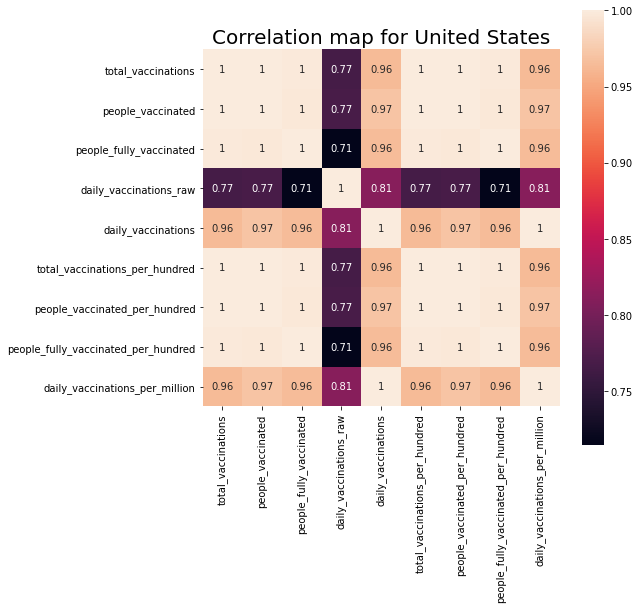
\includegraphics[scale=0.4]{../img/usa_corr.png} 
\caption{Korelacja pomiędzy atrybutami zbioru danych dla USA}
\end{figure}
\end{frame}

\begin{frame}{Państwa wiodące (stan na 25.05)}
\begin{enumerate}
\item<3-> Zjednoczone Emiraty Arabskie (75\%)
\item<1-> Izrael (59\%)
\item<4-> Chile (42\%)
\item<2-> Stany Zjednoczone (39\%)
\item<5-> Chiny (37\%)
\item<6-> Polska (16\%)
\end{enumerate}
\end{frame}

\begin{frame}{Algorytm predykcji}
\begin{figure}

\includegraphics[scale=0.4]{../img/regresja.jpg} 
\end{figure}
\end{frame}

\begin{frame}{Lepszy algorytm}
\begin{figure}

\includegraphics[scale=0.4]{../img/regresja2.jpg} 
\end{figure}
\end{frame}

\begin{frame}{Skuteczność regresji}
\begin{figure}[h!]
\centering
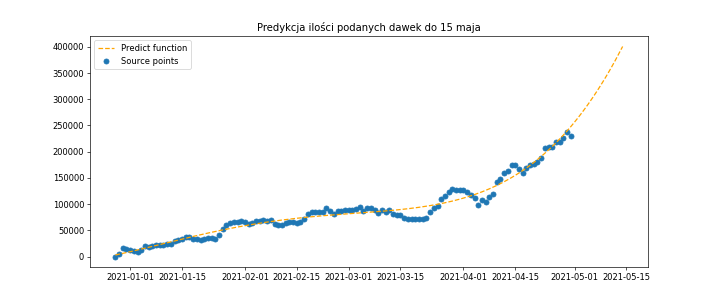
\includegraphics[scale=0.4]{../img/demand1.png} 
\caption{Ambitna predykcja programu szczepień w Polsce}
\label{Rys:poland}
\end{figure}
\end{frame}

\begin{frame}{Wnioski}
\begin{itemize}
\item dużo pracy wymagało wypełnienie brakujących wartości
\item algorytm przygotowywania danych można wykorzystać w przyszłości
\item łatwo można wskazać liderów w programach szczepień
\item algorytm regresji nie jest tutaj dobrym rozwiązaniem 
\item należy zbudować lepszy, bardziej złożony model
\end{itemize}
\end{frame}

\end{document}